\documentclass[aspectratio=169]{beamer}
\usepackage{hyperref}
\usepackage[T1]{fontenc}
\usepackage[spanish]{babel}
\usepackage{csquotes}
\usepackage{tribhuvan}

\usepackage{latexsym,amsmath,xcolor,multicol,booktabs,calligra}
\usepackage{graphicx,pstricks,listings,stackengine}

\author{Rodrigo Pérez Rodríguez}
\title{Tecnologías Robóticas para la Discapacidad Intelectual}
\subtitle{Sensores en robótica social y asistencial}
\date{}
\setbeamertemplate{date}{}

\AtBeginSection[]{
  \begin{frame}[plain]
    \vfill
    \begin{center}
      {\LARGE\bfseries \insertsectionhead}
    \end{center}
    \vfill
  \end{frame}
}
\AtBeginSubsection[]{}

% defs
\def\cmd#1{\texttt{\color{red}\footnotesize $\backslash$#1}}
\def\env#1{\texttt{\color{blue}\footnotesize #1}}
\definecolor{deepblue}{rgb}{0,0,0.5}
\definecolor{deepred}{rgb}{0.6,0,0}
\definecolor{deepgreen}{rgb}{0,0.5,0}
\definecolor{halfgray}{gray}{0.55}

\lstset{
    basicstyle=\ttfamily\small,
    keywordstyle=\bfseries\color{deepblue},
    emphstyle=\ttfamily\color{deepred},
    stringstyle=\color{deepgreen},
    numbers=left,
    numberstyle=\small\color{halfgray},
    rulesepcolor=\color{red!20!green!20!blue!20},
    frame=shadowbox,
}

\begin{document}

\begin{frame}
    \titlepage
\end{frame}

\begin{frame}
    \tableofcontents[sectionstyle=show,subsectionstyle=show/shaded/hide,subsubsectionstyle=show/shaded/hide]
\end{frame}

%=================================================
\section{Introducción}
%=================================================

\begin{frame}{Sistema de percepción del robot}
\small
\begin{itemize}
  \item Los sensores son dispositivos físicos que miden magnitudes del entorno o del propio robot.
  \item Ejemplos de magnitudes observables:
  \begin{itemize}
    \item distancia,
    \item sonido,
    \item magnetismo,
    \item presión,
    \item altitud.
  \end{itemize}
  \item La señal medida no equivale por sí sola al estado del robot ni a una interpretación semántica del entorno.
\end{itemize}
\end{frame}

\begin{frame}{De la medida al significado}
\small
\begin{itemize}
  \item Un sensor mide una magnitud, pero no proporciona directamente símbolos ni decisiones.
  \item Para transformar la medida en información útil intervienen varias disciplinas:
  \begin{itemize}
    \item \textbf{Electrónica:} por ejemplo, un sensor de colisión detecta si pasa o no corriente.
    \item \textbf{Procesamiento de señales:} un micrófono filtra ruido para captar la voz.
    \item \textbf{Computación:} un algoritmo sobre una cámara detecta la silueta de un objeto.
  \end{itemize}
  \item En robótica, percibir implica combinar medida física, procesamiento e interpretación.
\end{itemize}
\end{frame}

\begin{frame}{Integración de sensores}
\small
\begin{itemize}
  \item Normalmente no se diseña un sensor que resuelva por sí solo el problema final.
  \item Lo habitual es integrar información de sensores ya existentes.
  \item Ejemplos:
  \begin{itemize}
    \item detección de intrusos mediante temperatura, movimiento y otras pistas,
    \item medida de distancias mediante ultrasonidos, infrarrojos o visión estereoscópica.
  \end{itemize}
  \item La selección sensorial condiciona coste, robustez, alcance y complejidad del procesamiento posterior.
\end{itemize}
\end{frame}

%=================================================
\section{Caracterización de los sensores}
%=================================================

\begin{frame}{Parámetros básicos de caracterización}
\small
\begin{itemize}
  \item \textbf{Sensibilidad:} tasa de cambio de la salida cuando cambia la entrada.
  \item \textbf{Linealidad:} constancia de la relación entre entrada y salida.
  \item \textbf{Rango:} diferencia entre el valor máximo y el mínimo medible.
  \item \textbf{Tiempo de respuesta:} tiempo necesario para observar un cambio en la entrada.
  \item \textbf{Exactitud:} diferencia entre el valor real y el medido.
  \item \textbf{Resolución:} incremento mínimo observable en la entrada.
  \item \textbf{Repetitividad:} variación entre medidas sucesivas sobre la misma entrada.
  \item \textbf{Tipo de salida:} entero, real, vector, matriz, etc.
\end{itemize}
\end{frame}

\begin{frame}{Por qué importa esta caracterización}
\small
\begin{itemize}
  \item Dos sensores que miden la misma magnitud pueden tener comportamientos muy distintos.
  \item La caracterización permite decidir si un sensor sirve para control, supervisión o percepción de alto nivel.
  \item En robótica asistencial, estos parámetros condicionan:
  \begin{itemize}
    \item seguridad,
    \item robustez frente al ruido,
    \item frecuencia de actualización,
    \item fiabilidad clínica o educativa.
  \end{itemize}
\end{itemize}
\end{frame}

\begin{frame}{Calibración: condición para una medida fiable}
\small
\begin{itemize}
  \item Todo sensor introduce errores sistemáticos: sesgo, escala y ruido.
  \item \textbf{Calibración intrínseca:} ajusta parámetros propios del sensor.
  \item \textbf{Calibración extrínseca:} estima la posición y orientación del sensor respecto al robot.
  \item Sin calibración adecuada, la percepción puede degradarse aunque el hardware sea de calidad.
  \item En robótica asistencial esto impacta directamente en seguridad y robustez de la interacción.
\end{itemize}
\end{frame}

\begin{frame}{Sincronización y fusión sensorial}
\small
\begin{itemize}
  \item La percepción real combina datos de múltiples sensores con distinta frecuencia y latencia.
  \item Dos requisitos básicos para fusionar:
  \begin{itemize}
    \item coherencia \textbf{espacial} (mismo marco de referencia),
    \item coherencia \textbf{temporal} (medidas alineadas en el tiempo).
  \end{itemize}
  \item Si no hay sincronización, pueden aparecer falsas detecciones o estimaciones inestables.
  \item Diseñar la sensórica implica diseñar también su calibración, temporización y estrategia de fusión.
\end{itemize}
\end{frame}

%=================================================
\section{Clasificación}
%=================================================

\begin{frame}{Clasificación por localización}
\small
\begin{itemize}
  \item \textbf{Internos al robot:}
  \begin{itemize}
    \item posición,
    \item velocidad,
    \item aceleración.
  \end{itemize}
  \item \textbf{Externos al robot:}
  \begin{itemize}
    \item proximidad,
    \item tacto,
    \item fuerza,
    \item visión.
  \end{itemize}
  \item Esta distinción separa la percepción del propio cuerpo del robot y la observación del entorno.
\end{itemize}
\end{frame}

\begin{frame}{Clasificación por principio de operación}
\small
\begin{itemize}
  \item \textbf{Sensores pasivos:} miden señales presentes en el entorno.
  \begin{itemize}
    \item interruptores,
    \item sensores de luz,
    \item botones.
  \end{itemize}
  \item \textbf{Sensores activos:} generan un estímulo y miden su interacción con el entorno.
  \begin{itemize}
    \item ultrasonidos,
    \item infrarrojos,
    \item láser.
  \end{itemize}
  \item Los activos suelen exigir más energía y más procesamiento, pero ofrecen más capacidad de observación.
\end{itemize}
\end{frame}

%=================================================
\section{Tipos de sensores}
%=================================================

\begin{frame}{Sensores de interruptor}
\small
\begin{itemize}
  \item Sensor pasivo.
  \item Puede emplearse de forma interna o externa.
  \item Requiere poco procesamiento.
  \item Usos frecuentes:
  \begin{itemize}
    \item detectar contacto o colisión,
    \item marcar límites mecánicos,
    \item realizar conteos por apertura o cierre.
  \end{itemize}
\end{itemize}
\end{frame}

\begin{frame}{Sensores de tacto}
\small
\begin{columns}[T,onlytextwidth]
  \begin{column}{0.58\textwidth}
    \begin{itemize}
      \item Sensor pasivo y externo.
      \item Permite estimar el perfil o el contacto con un objeto.
      \item Puede entenderse como una extensión del sensor de interruptor.
      \item Ejemplos de implementación:
      \begin{itemize}
        \item dedo sensorizado,
        \item púas,
        \item bigotes táctiles.
      \end{itemize}
    \end{itemize}
  \end{column}
  \begin{column}{0.42\textwidth}
    \centering
    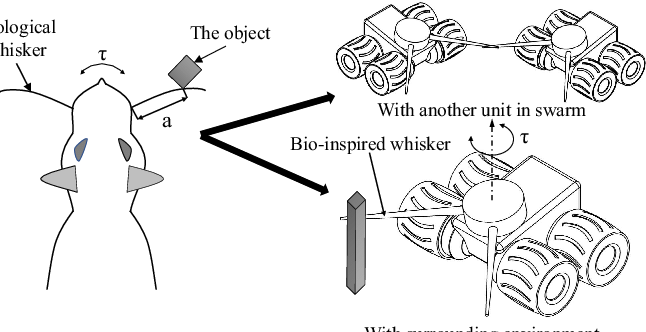
\includegraphics[width=0.97\linewidth,height=0.62\textheight,keepaspectratio]{images/tema_2/s12_sensores-de-tacto_img01.png}
  \end{column}
\end{columns}
\end{frame}

\begin{frame}{Sensores de posición}
\small
\begin{columns}[T,onlytextwidth]
  \begin{column}{0.58\textwidth}
    \begin{itemize}
      \item Sensores pasivos e internos.
      \item Indican la posición de un elemento del robot, por ejemplo una articulación.
      \item Pueden ser rotacionales o traslacionales.
      \item Tipos habituales:
      \begin{itemize}
        \item eléctricos, como potenciómetros,
        \item ópticos, como optointerruptores.
      \end{itemize}
    \end{itemize}
  \end{column}
  \begin{column}{0.42\textwidth}
    \centering
    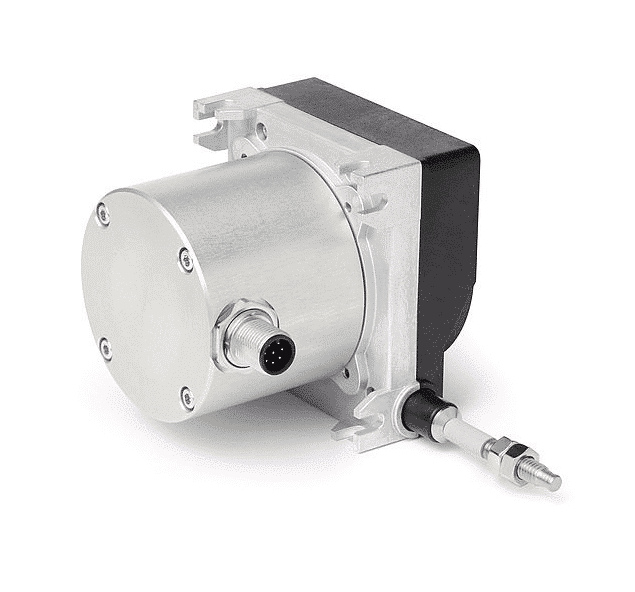
\includegraphics[width=0.97\linewidth,height=0.62\textheight,keepaspectratio]{images/tema_2/s13_sensores-de-posicion_img01.png}
  \end{column}
\end{columns}
\end{frame}

\begin{frame}{Sensores de luz ambiente}
\small
\begin{columns}[T,onlytextwidth]
  \begin{column}{0.60\textwidth}
    \begin{itemize}
      \item Sensores pasivos y externos.
      \item Su resistencia varía en función de la luz incidente.
      \item Son muy sensibles a la colocación física y a las condiciones del entorno.
      \item Resultan útiles para tareas simples, pero requieren cuidado en calibración y montaje.
    \end{itemize}
  \end{column}
  \begin{column}{0.40\textwidth}
    \centering
    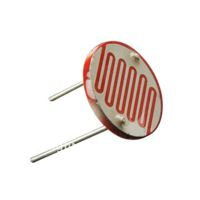
\includegraphics[width=0.90\linewidth,height=0.48\textheight,keepaspectratio]{images/tema_2/s14_sensores-de-luz-ambiente_img01.jpeg}
  \end{column}
\end{columns}
\end{frame}

\begin{frame}{Fotosensores activos}
\small
\begin{itemize}
  \item Están formados por un emisor y un receptor.
  \item Habitualmente:
  \begin{itemize}
    \item el emisor es un LED,
    \item el receptor es un fotodiodo o un fototransistor.
  \end{itemize}
  \item Según su disposición:
  \begin{itemize}
    \item \textbf{reflexión,} cuando emisor y receptor están juntos,
    \item \textbf{barrera,} cuando el haz se interrumpe entre ambos.
  \end{itemize}
  \item Aplicaciones: detección de obstáculos, medida de distancia, seguimiento de línea o lectura de códigos de barras.
\end{itemize}
\end{frame}

\begin{frame}{Limitaciones de los fotosensores activos}
\small
\begin{itemize}
  \item La reflexión depende del color y de las propiedades del material.
  \item En general, los objetos claros reflejan más que los oscuros.
  \item Consecuencias prácticas:
  \begin{itemize}
    \item es menos fiable detectar objetos oscuros,
    \item los claros pueden parecer más cercanos y los oscuros más lejanos.
  \end{itemize}
  \item La luz ambiente introduce ruido, por lo que suele ser necesaria calibración periódica.
\end{itemize}
\end{frame}

\begin{frame}{Sensores de infrarrojos}
\small
\begin{itemize}
  \item Son sensores de luz en el espectro infrarrojo.
  \item Para distinguir la señal útil del infrarrojo ambiente suele emplearse modulación.
  \item Son activos: combinan emisor y receptor.
  \item Se usan tanto en reflexión como en barrera.
  \item Ventajas y limitaciones:
  \begin{itemize}
    \item son muy comunes y fácilmente modulables,
    \item no son visibles,
    \item algunos objetos reflejan mal el infrarrojo,
    \item la intensidad decrece rápidamente con la distancia.
  \end{itemize}
\end{itemize}
\end{frame}

\begin{frame}{Sensores de rotación}
\small
\begin{columns}[T,onlytextwidth]
  \begin{column}{0.60\textwidth}
    \begin{itemize}
      \item Miden rotación angular.
      \item Aplicaciones típicas:
      \begin{itemize}
        \item odometría, para contar vueltas,
        \item velocimetría, para estimar velocidad angular.
      \end{itemize}
      \item Es habitual marcar el elemento que gira para contar eventos de paso.
      \item La resolución depende del patrón utilizado:
      \begin{itemize}
        \item un único marcador da baja resolución,
        \item múltiples marcas mejoran resolución, pero exigen más velocidad de lectura.
      \end{itemize}
    \end{itemize}
  \end{column}
  \begin{column}{0.40\textwidth}
    \centering
    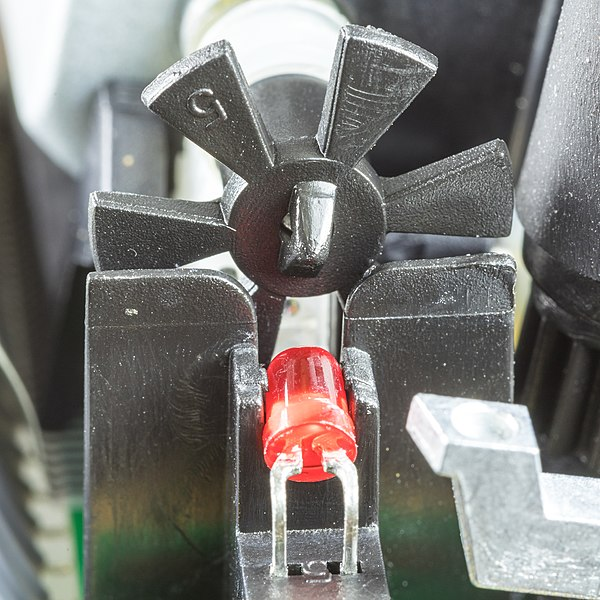
\includegraphics[width=0.97\linewidth,height=0.52\textheight,keepaspectratio]{images/tema_2/s18_sensores-de-rotacion_img01.jpeg}
  \end{column}
\end{columns}
\end{frame}

\begin{frame}{Sensores de velocidad}
\small
\begin{itemize}
  \item Sensores pasivos e internos.
  \item Miden normalmente velocidad angular.
  \item Implementaciones frecuentes:
  \begin{itemize}
    \item \textbf{eléctricas:} una bobina gira perpendicularmente a un campo magnético y genera una tensión proporcional,
    \item \textbf{ópticas:} se combinan sensores de posición con temporizadores.
  \end{itemize}
\end{itemize}
\end{frame}

\begin{frame}{Sensores de aceleración}
\small
\begin{columns}[T,onlytextwidth]
  \begin{column}{0.58\textwidth}
    \begin{itemize}
      \item Sensores pasivos e internos.
      \item Miden aceleración lineal del robot o de alguno de sus elementos.
      \item Son clave para estimar movimiento, vibraciones o inclinación.
      \item En plataformas reales suelen combinarse con otros sensores para mejorar la estimación de estado.
    \end{itemize}
  \end{column}
  \begin{column}{0.42\textwidth}
    \centering
    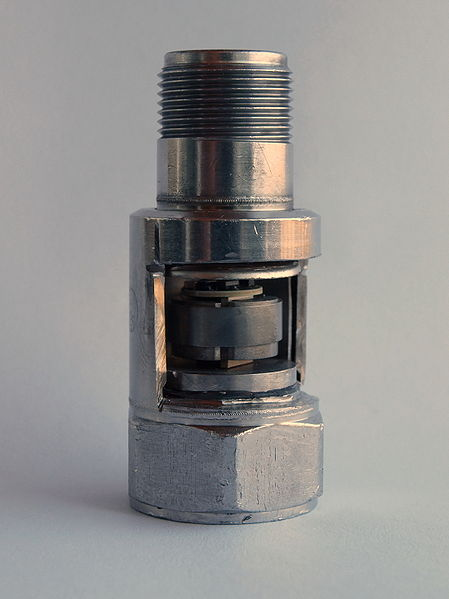
\includegraphics[width=0.88\linewidth,height=0.60\textheight,keepaspectratio]{images/tema_2/s20_sensores-de-aceleracion_img01.jpeg}
  \end{column}
\end{columns}
\end{frame}

\begin{frame}{Sensores inerciales}
\small
\begin{columns}[T,onlytextwidth]
  \begin{column}{0.58\textwidth}
    \begin{itemize}
      \item Sensores pasivos e internos.
      \item La instrumentación inercial combina acelerómetros, giróscopos y magnetómetros.
      \item Permiten medir aceleración y velocidad angular.
      \item Problema habitual: las oscilaciones mecánicas pueden producir medidas falsas o degradadas.
    \end{itemize}
  \end{column}
  \begin{column}{0.42\textwidth}
    \centering
    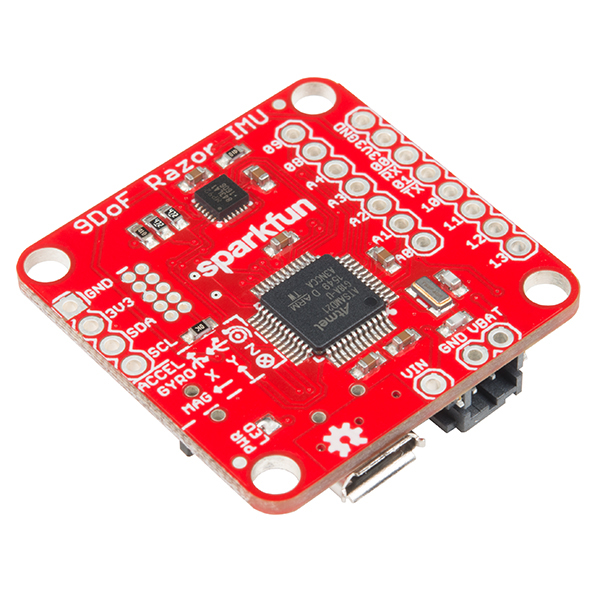
\includegraphics[width=0.97\linewidth,height=0.58\textheight,keepaspectratio]{images/tema_2/s21_sensores-inerciales_img01.jpeg}
  \end{column}
\end{columns}
\end{frame}

\begin{frame}{Sensores de ultrasonidos}
\small
\begin{columns}[T,onlytextwidth]
  \begin{column}{0.58\textwidth}
    \begin{itemize}
      \item Se utilizan sobre todo para medir distancias.
      \item El emisor genera un ultrasonido y el receptor capta su eco reflejado.
      \item Son una solución extendida por sencillez y coste moderado.
    \end{itemize}
  \end{column}
  \begin{column}{0.42\textwidth}
    \centering
    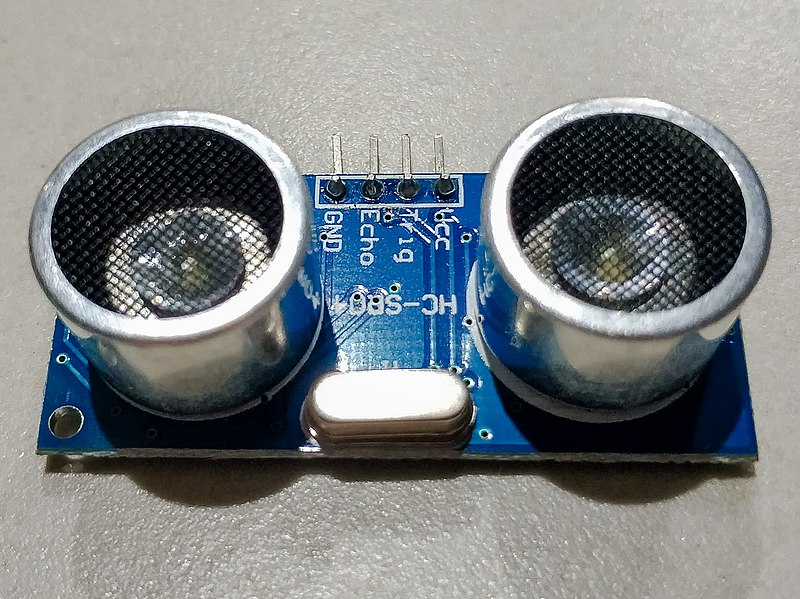
\includegraphics[width=0.97\linewidth,height=0.50\textheight,keepaspectratio]{images/tema_2/s22_sensores-de-us_img01.jpeg}
  \end{column}
\end{columns}
\end{frame}

\begin{frame}{Limitaciones de los ultrasonidos}
\small
\begin{itemize}
  \item La medida informa de una distancia, pero no de la posición exacta del objeto.
  \item Existen reflejos especulares dependientes del ángulo de incidencia.
  \item Las superficies pulidas son problemáticas; las rugosas generan respuestas distintas.
  \item Los errores suelen crecer con la distancia al objeto.
\end{itemize}
\end{frame}

\begin{frame}{Sensores láser}
\small
\begin{itemize}
  \item Comparten con los ultrasonidos la idea de medir tiempo de eco.
  \item Ofrecen mucha más precisión.
  \item El caso más representativo es el \textbf{LiDAR}, basado en láser pulsado.
  \item Son fundamentales en navegación, mapeado y evitación de obstáculos.
\end{itemize}
\vspace{1mm}
\begin{columns}[T,onlytextwidth]
  \begin{column}{0.40\textwidth}
    \centering
    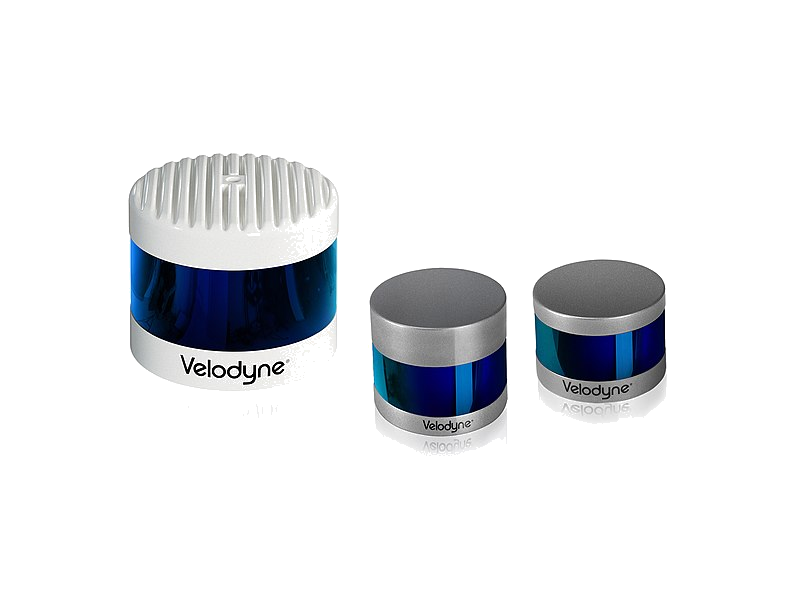
\includegraphics[width=0.90\linewidth,height=0.24\textheight,keepaspectratio]{images/tema_2/s24_sensores-laser_img01.png}
  \end{column}
  \begin{column}{0.60\textwidth}
    \centering
    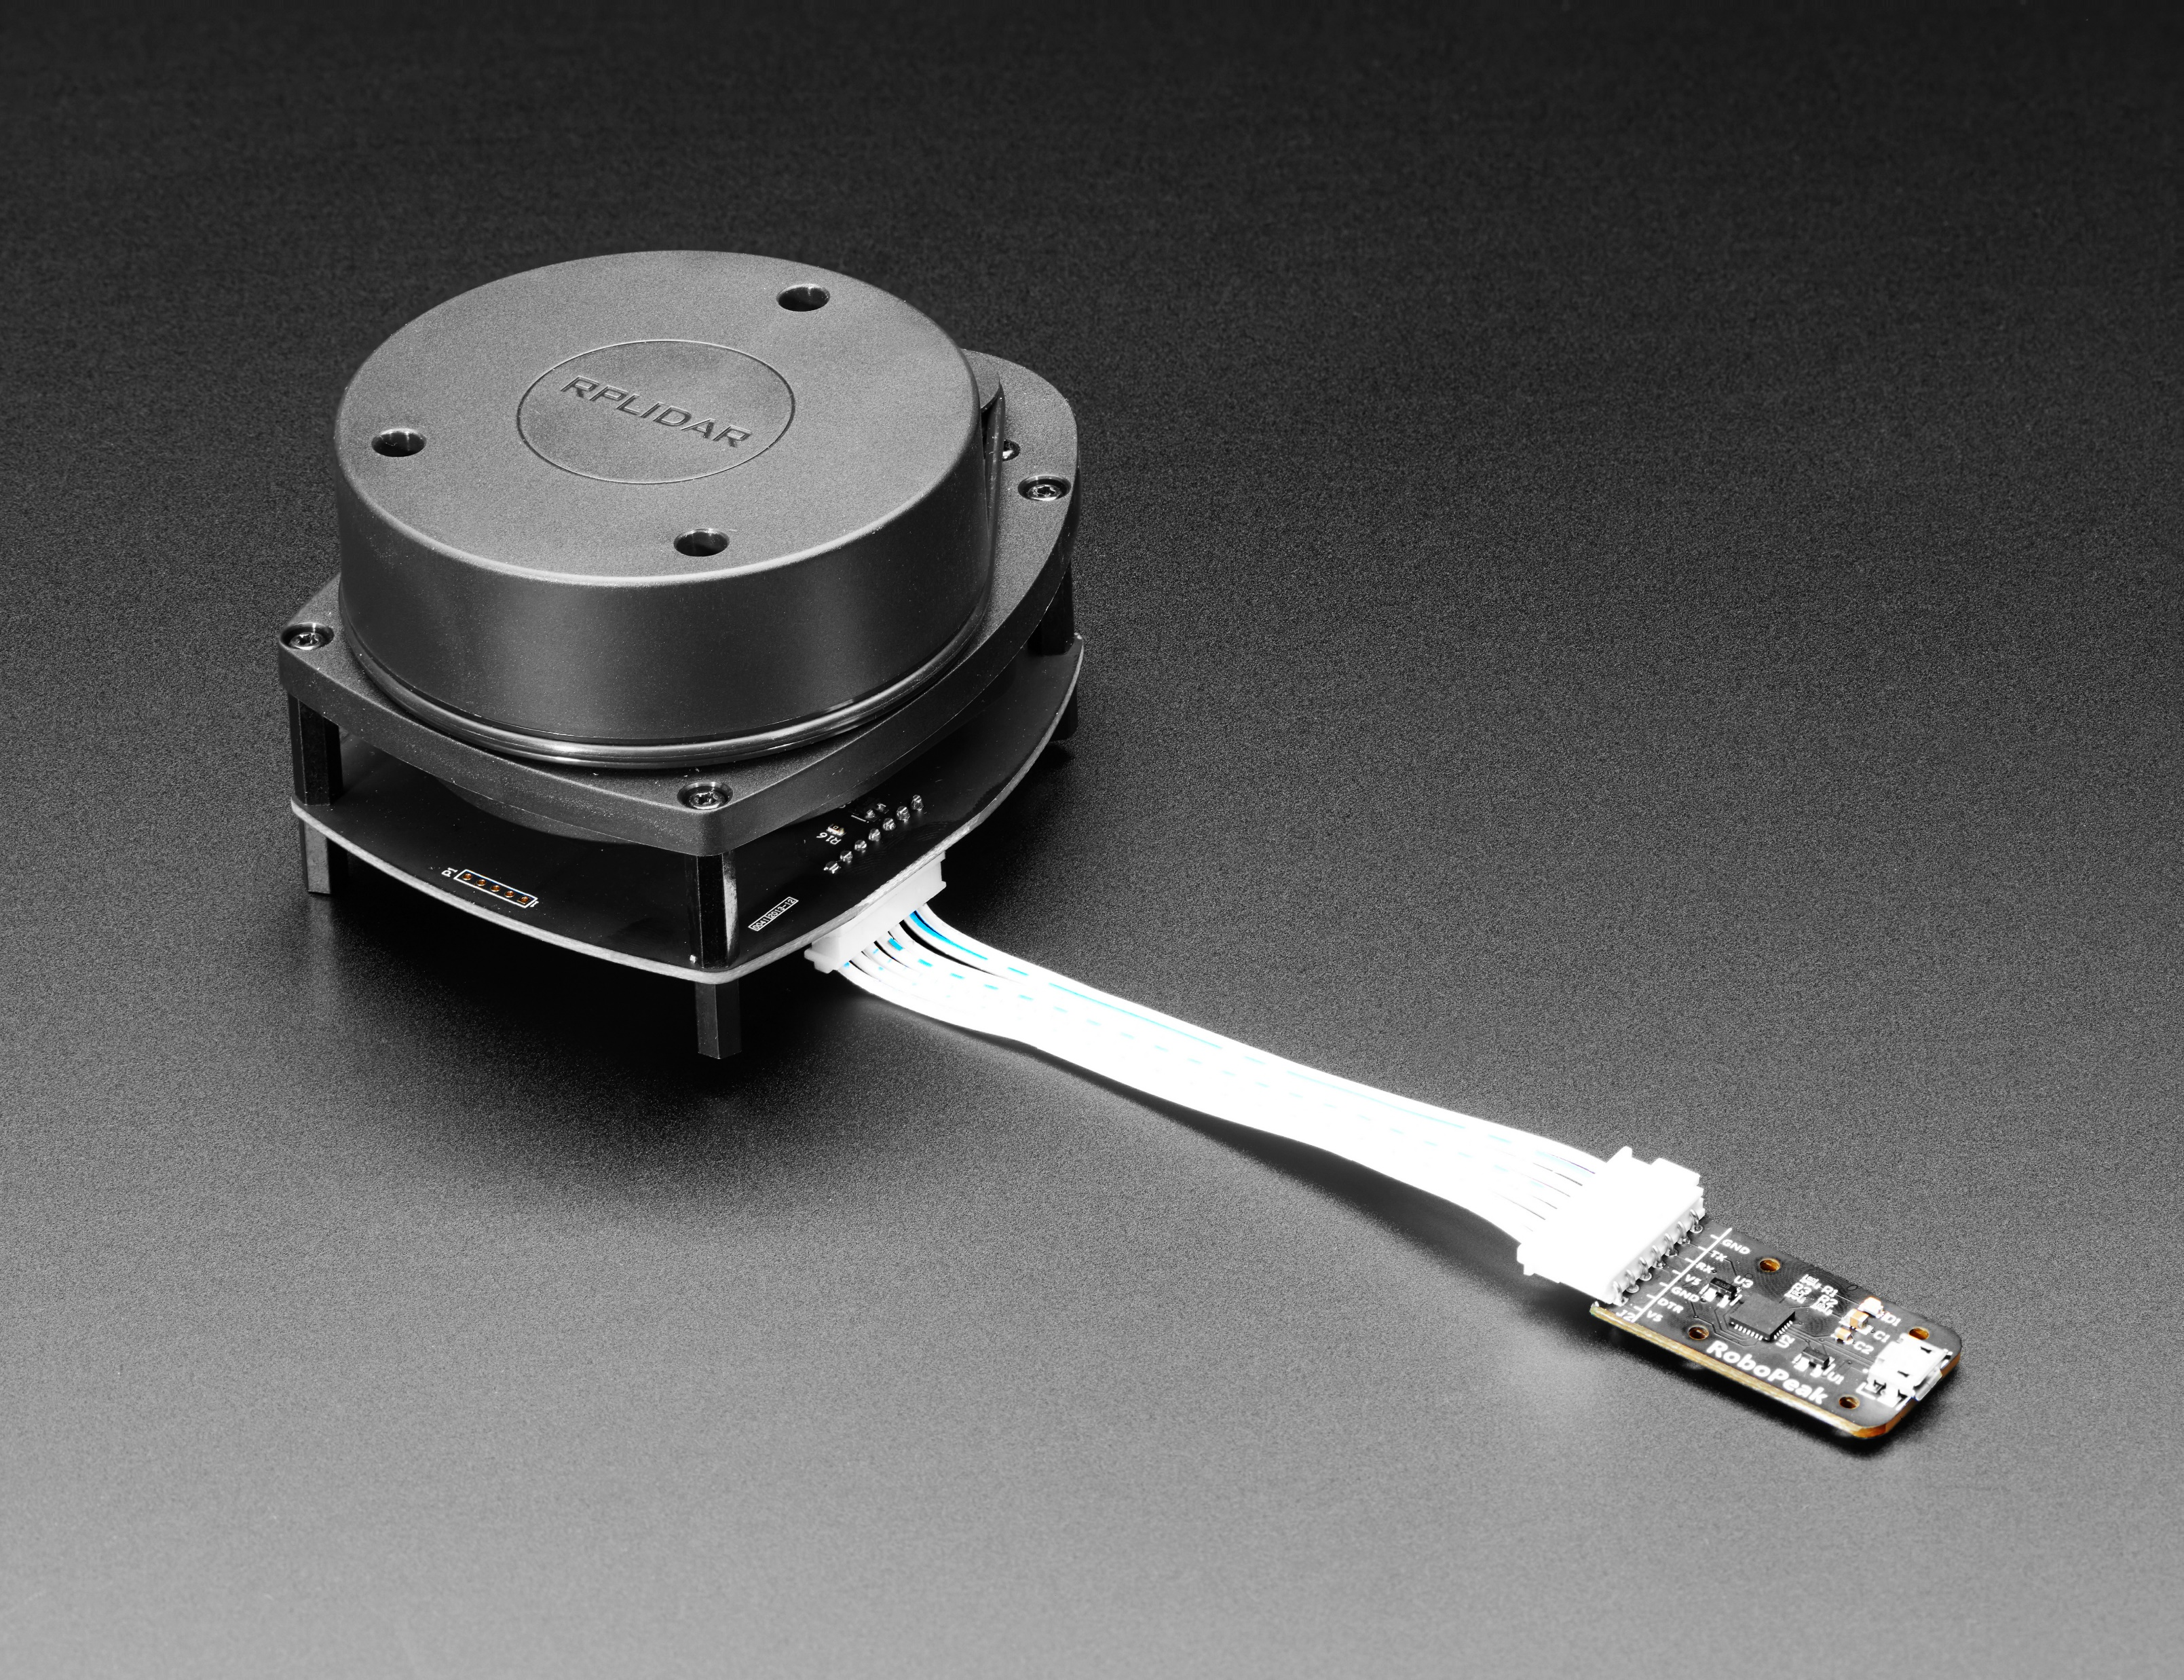
\includegraphics[width=0.97\linewidth,height=0.24\textheight,keepaspectratio]{images/tema_2/s24_sensores-laser_img02.jpeg}
  \end{column}
\end{columns}
\end{frame}

\begin{frame}{Cámaras}
\small
\begin{columns}[T,onlytextwidth]
  \begin{column}{0.58\textwidth}
    \begin{itemize}
      \item Son sensores de luz y constituyen la base de la visión artificial.
      \item Tecnologías habituales: CCD y CMOS.
      \item Variantes comunes: blanco y negro, color e infrarrojo.
      \item Suelen diferenciarse por resolución y tasa de imágenes por segundo.
      \item Ventajas e inconvenientes:
      \begin{itemize}
        \item aportan gran riqueza informativa,
        \item extraer información útil puede ser complejo,
        \item generan grandes volúmenes de datos.
      \end{itemize}
    \end{itemize}
  \end{column}
  \begin{column}{0.42\textwidth}
    \centering
    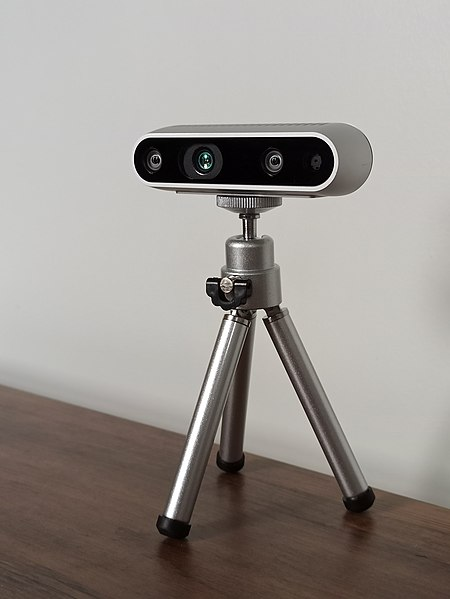
\includegraphics[width=0.85\linewidth,height=0.60\textheight,keepaspectratio]{images/tema_2/s25_camaras_img01.jpeg}
  \end{column}
\end{columns}
\end{frame}

\begin{frame}{Cámaras RGBD y ToF}
\small
\begin{columns}[T,onlytextwidth]
  \begin{column}{0.58\textwidth}
    \begin{itemize}
      \item \textbf{RGBD:}
      \begin{itemize}
        \item ejemplos: Kinect v1, Xtion,
        \item usan luz infrarroja estructurada o estereoscopía,
        \item producen nube de puntos e imagen de profundidad,
        \item su alcance típico es inferior a 6 m.
      \end{itemize}
      \item \textbf{ToF:}
      \begin{itemize}
        \item ejemplos: Kinect2, PointGrey,
        \item emiten láser pulsado y miden tiempo de vuelo,
        \item alcanzan distancias inferiores a 8 m,
        \item proporcionan medidas muy precisas.
      \end{itemize}
    \end{itemize}
  \end{column}
  \begin{column}{0.42\textwidth}
    \centering
    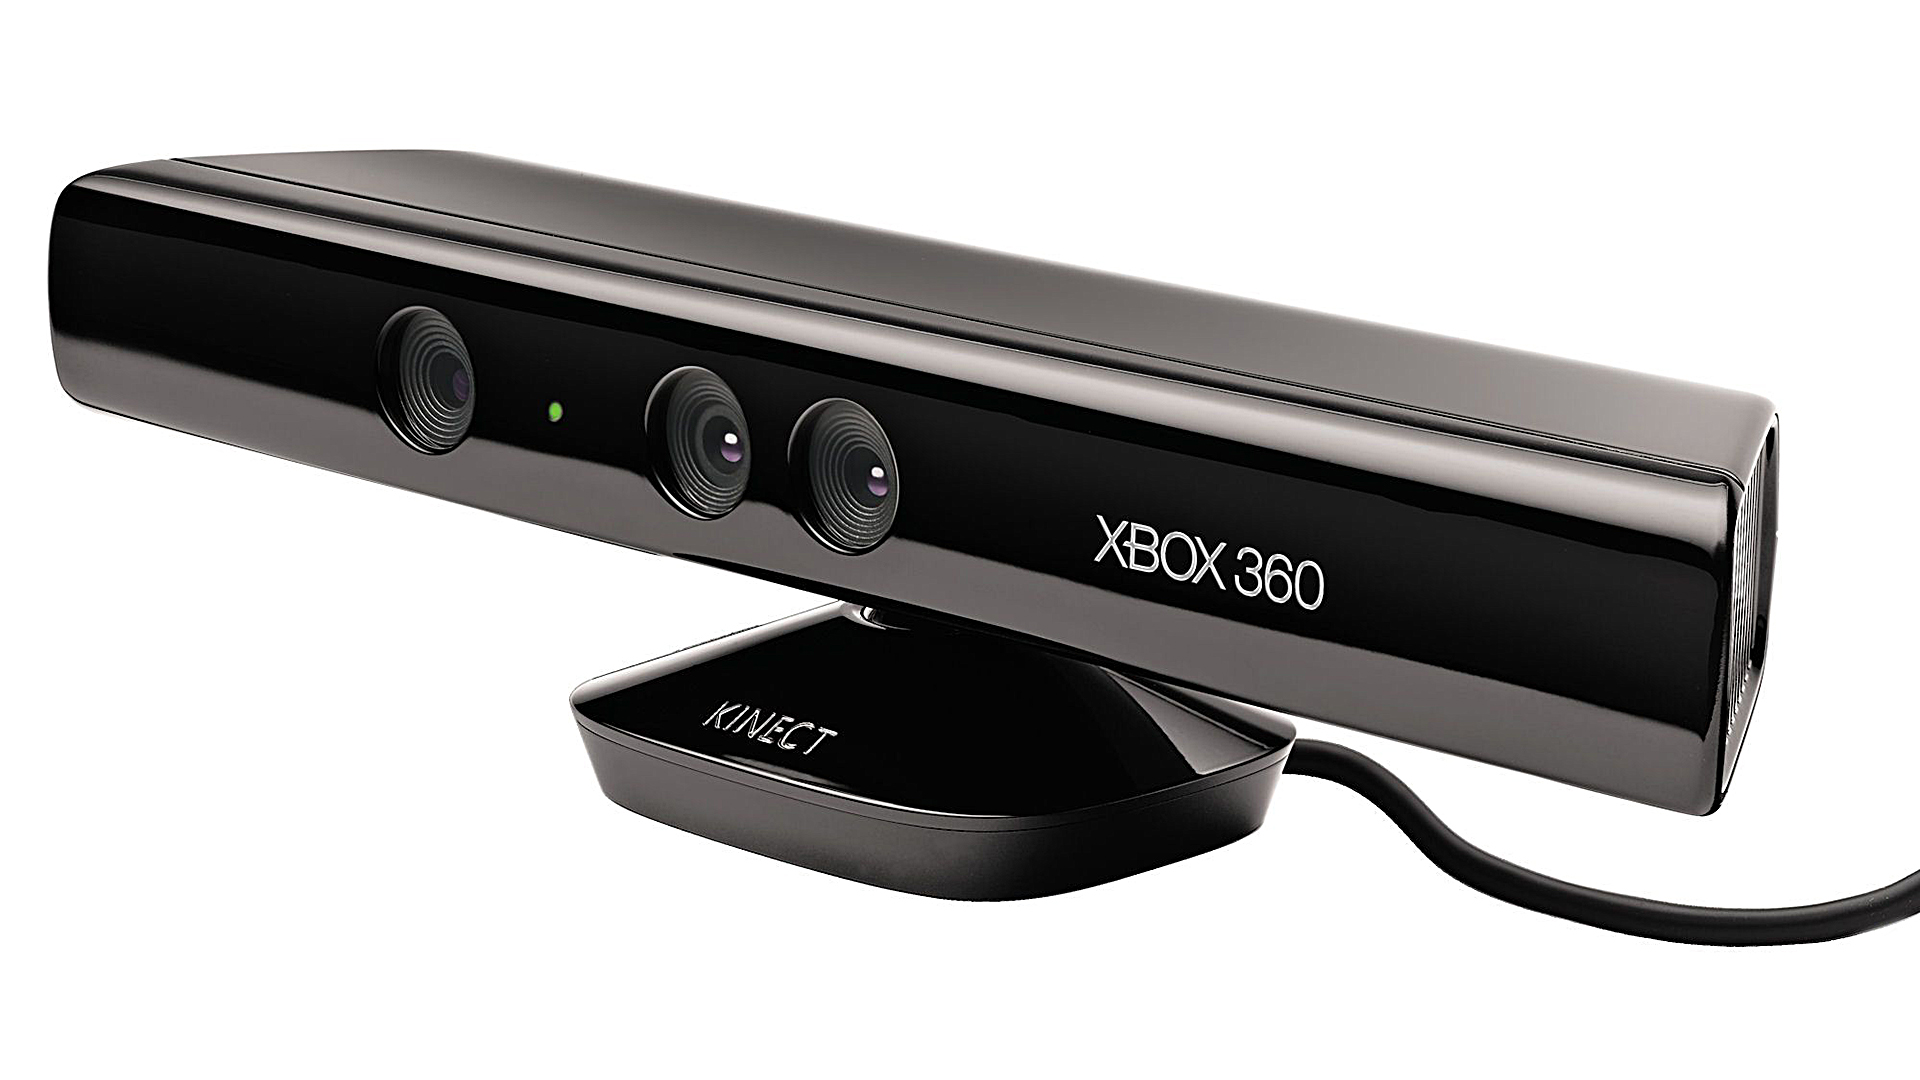
\includegraphics[width=0.97\linewidth,height=0.42\textheight,keepaspectratio]{images/tema_2/s26_camaras_img01.jpeg}
  \end{column}
\end{columns}
\end{frame}

\begin{frame}{Conclusión}
\small
\begin{itemize}
  \item No existe un sensor universal: cada tecnología impone compromisos entre coste, alcance, resolución y robustez.
  \item En robótica social y asistencial, la percepción fiable depende de combinar sensores, calibración y procesamiento.
  \item Elegir bien la sensórica es una decisión arquitectónica que condiciona el comportamiento global del robot.
\end{itemize}
\end{frame}

\end{document}